\documentclass{article}

\usepackage{graphicx}
\usepackage{tikz}
\usepackage{tikzsymbols}
\usetikzlibrary{calc,patterns,shapes.geometric}
\pagestyle{empty}
\usepackage[margin=0pt]{geometry}
\geometry{papersize={14in,12in}}

\def\centerarc[#1](#2)(#3:#4:#5){\draw[#1] ($(#2)+({#5*cos(#3)},{#5*sin(#3)})$) arc (#3:#4:#5);}

\begin{document}
	\begin{figure}
		\centering
		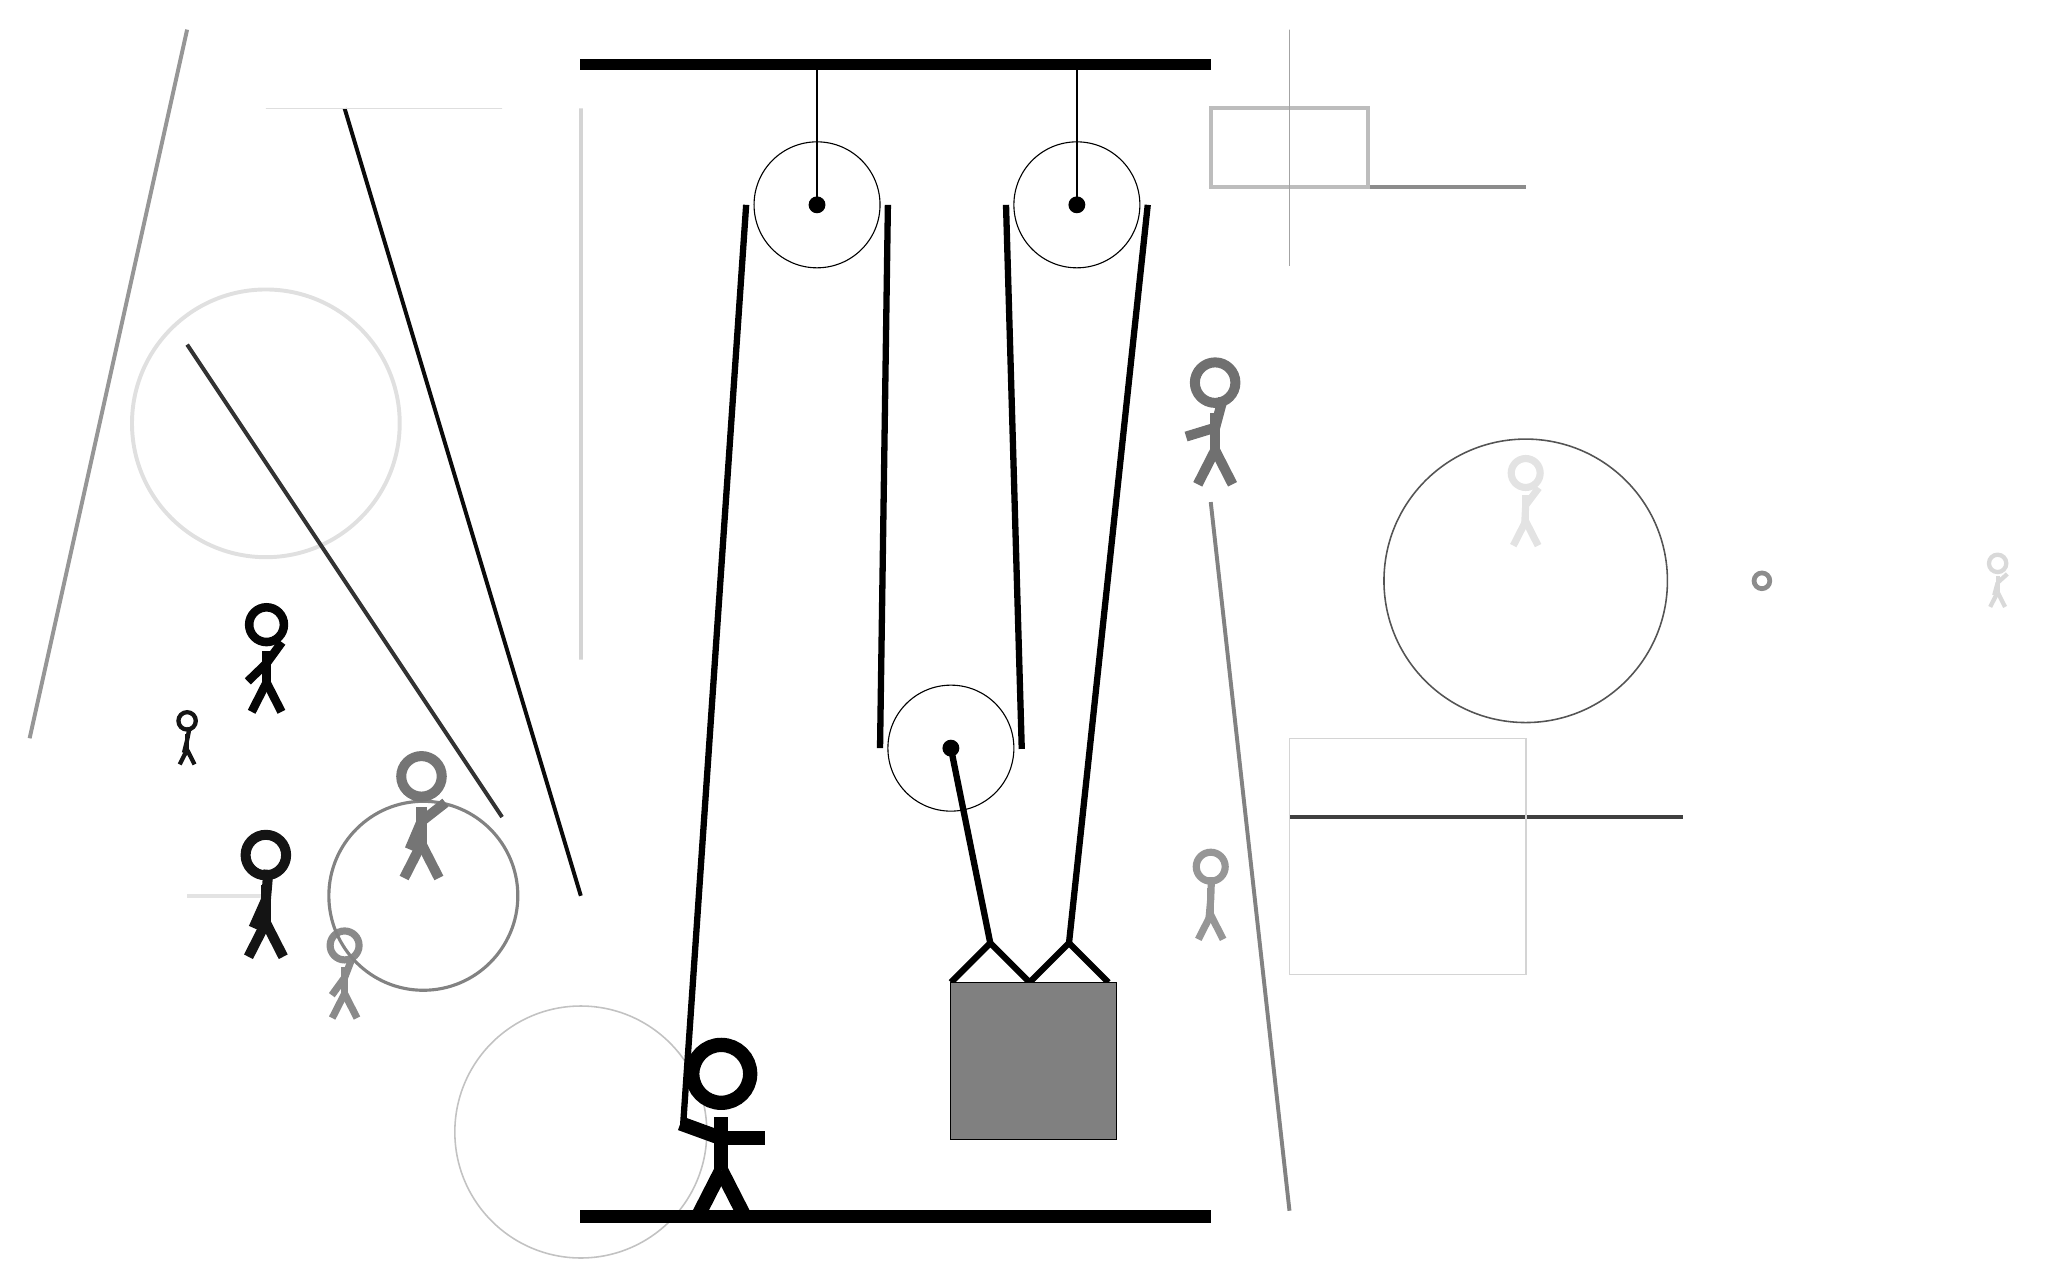
\begin{tikzpicture}
			%%%%% START %%%%%
			
			\draw[fill=black] (-2, 11.5) rectangle (6, 11.625);
			
			\draw (1, 9.775) circle (0.8);
			\draw[fill=black] (1, 9.775) circle (0.1);
			\draw[thick] (1, 9.775) -- (1, 11.5);
			
			\draw (4.3, 9.775) circle (0.8);
			\draw[fill=black] (4.3, 9.775) circle (0.1);
			\draw[thick] (4.3, 9.775) -- (4.3, 11.5);
			
			\draw (2.7, 2.875) circle (0.8);
			\draw[fill=black] (2.7, 2.875) circle (0.1);
			
			\draw[line width=0.8mm]  (2.7, -0.1) -- (3.2, 0.4) -- (3.7, -0.1) -- (4.2, 0.4) -- (4.7, -0.1);
			\draw[fill=black!50] (2.7, -0.1) rectangle (4.8, -2.1);
			
			\node[line width=0.4mm, color=black!98] at (-6, 4) {\Strichmaxerl[6][44][54]};
			
			\draw[line width=0.5mm, color=black!11](-7, 1) -- (-6, 1);
			\draw[line width=0.5mm, color=black!45](10, 10) -- (6, 10);
			\node[line width=0.5mm, color=black!92] at (-7, 3) {\Strichmaxerl[3][76][79]};
			
			\draw [line width=0.2mm, color=black!67](10, 5) circle (1.8);
			\draw[line width=0.5mm, color=black!26] (6, 11) rectangle (8, 10);
			\draw[line width=0.5mm, color=black!96](-2, 1) -- (-5, 11);
			
			\draw[line width=0.2mm, color=black!13] (-3, 11) rectangle (-6, 11);
			\node[line width=0.4mm, color=black!15] at (16, 5) {\Strichmaxerl[3][75][42]};
			
			\draw[line width=0.5mm, color=black!49](6, 6) -- (7, -3);
			
			\draw [line width=0.5mm, color=black!12](-6, 7) circle (1.7);
			\node[line width=0.7mm, color=black!46] at (-5, 0) {\Strichmaxerl[5][54][69]};
			\draw[line width=0.5mm, color=black!75](7, 2) -- (12, 2);
			
			\draw[line width=0.2mm, color=black!17] (7, 3) rectangle (10, 0);
			\draw [line width=0.4mm, color=black!49](-4, 1) circle (1.2);
			\draw [line width=0.6mm, color=black!45](13, 5) circle (0.1);
			
			\node[line width=0.3mm, color=black!41] at (6, 1) {\Strichmaxerl[5][85][88]};
			
			\draw[line width=0.2mm, color=black!36] (7, 9) rectangle (7, 12);
			\node[line width=0.2mm, color=black!54] at (-4, 2) {\Strichmaxerl[7][67][38]};
			\draw[line width=0.5mm, color=black!41](-7, 12) -- (-9, 3);
			\node[line width=0.7mm, color=black!11] at (10, 6) {\Strichmaxerl[5][87][53]};
			\draw[line width=0.5mm, color=black!80](-3, 2) -- (-7, 8);
			\node[line width=0.2mm, color=black!92] at (-6, 1) {\Strichmaxerl[7][66][85]};
			\node[line width=0.3mm, color=black!56] at (6, 7) {\Strichmaxerl[7][17][75]};
			\draw[line width=0.5mm, color=black!17] (-2, 4) rectangle (-2, 11);
			
			\draw [line width=0.2mm, color=black!24](-2, -2) circle (1.6);
			
			\draw[line width=0.8mm](-0.7, -1.9) -- (0.1, 9.775);
			\centerarc[line width=0.8mm](1, 9.775)(0:180:0.9);
			\draw[line width=0.8mm](1.9, 9.775) -- (1.8, 2.875);
			\centerarc[line width=0.8mm](2.7, 2.875)(180:370:0.9);
			\draw[line width=0.8mm] (3.6, 2.865) -- (3.4, 9.775);
			\centerarc[line width=0.8mm](4.3, 9.775)(0:180:0.9);
			\draw[line width=0.8mm](4.2, 0.4) -- (5.2, 9.775);
			\draw[line width=0.8mm] (3.2, 0.4) -- (2.7, 2.875);
			
			\node at (-0.2, -2) {\Strichmaxerl[10][-20][0]};
			
			\draw[fill=black] (-2, -3) rectangle (6, -3.15);
			
			%%%%% END %%%%%
		\end{tikzpicture}
	\end{figure}	
\end{document}